\section{Risk identification and assessment}

In this section risk identification and assessment is provided by taking into account the defined data of the previous sections. Here it is also provided the information about the revised-risks. 

The factors that have been used in the identification process are: enterprise environmental factors, organizational process assets, the project scope statement and the project management plan.

It is worth to mention that after analysing these points, risks have been classified in two main groups: External risks, which are risks the project team cannot control and therefore no response nor action can be defined, and Internal risks, which can be detected in advance and be addressed properly.

Table \ref{risk_identification_and_assessment} presents the following information for each risk:

\begin{itemize}
	\item Probability to happen
	\item Impact regarding quality, time and cost
	\item Score using the weights of section \ref{3.4}
	\item Response. What is going to be done in order to avoid the risk before it happens.
\end{itemize}

Note that there are different types of responses that have been classified in these groups:

\begin{itemize}
	\item Mitigation. Actions to reduce the severity, seriousness, or painfulness of the risk.
	\item Transfer. Delegation of the actions to an outsourced company.
	\item Avoidance. Actions to keep away the risk and to avoid it.
	\item Acceptance. A difficult or unpleasant situation is accepted and a response is done in order to solve the issue.
\end{itemize}

\begin{landscape}
%\vspace*{\fill}

	\begin{longtable}{| >{\raggedright\arraybackslash}p{1.4cm} | >{\raggedright\arraybackslash}p{4cm} | >{\raggedright\arraybackslash}p{2cm} | >{\centering\arraybackslash}p{3cm} | >{\centering\arraybackslash}p{2cm} | >{\centering\arraybackslash}p{1.4cm} | >{\centering\arraybackslash}p{1.5cm} | >{\raggedright\arraybackslash}p{4cm} | }
		
		\toprule [2pt]

		\multirow{2}{*}{\textbf{Risk ID}}   &  \multirow{2}{*}{\textbf{Risk Statement}}   &	  \multirow{2}{*}{\textbf{Probability}}   &     \multicolumn{3}{| c |}{\textbf{Impact}} &  \multirow{2}{*}{ \textbf{Score}}  &    \multirow{2}{*}{\textbf{Response}}   \\
		
		\cline{4-6}

		\multirow{2}{*}{}  &   \multirow{2}{*}{}  &  \multirow{2}{*}{}  &  \textbf{Scope/Quality}  &   \textbf{Schedule}  &   \textbf{Cost}  &    \multirow{2}{*}{}  & \multirow{2}{*}{}   \\  

		\midrule [1.5pt]
		\endhead

		
		R.1 & Deliverable delays  & Medium   &  1  &  4   & 3  &  1.6  & Mitigation: Dedicate more resources than expected. \\  

		\hline
		
		R.2 & Inaccurate cost forecast  &  High  & 3  &   2  &  4  & 2.6 & Transfer: Consider new
		funding sources and revise
		the financial management plan.
		 \\  

		\hline
		
		R.3 & Lack of communication  & High   &  3  &   4  & 3  & 2.6 & Avoidance: Periodical meetings and use of collaborative software. \\  

		\hline
		
		R.4 & Lack of technology improvement  & Low   &  3  & 2    &  1  &  0.7   & Avoidance: Guarantee the development with thorough search of the actual technology. \\  

		\hline

		R.5 & Lack of access to project needed information  &  Very Low  &  2  &  2   & 2  & 0.4  & Avoidance: A previous accurate research is needed before the development of the project.  \\  

		\hline

		R.6 & Low team motivation  &  Medium  & 3  &   5  &  1  & 1.4  & Acceptance: Personal control and team building projects. \\  

		\hline

		R.7 & Unsuccessfully quality control   &  Low  & 4  &   2  & 2  & 1.0  &  Mitigation: Improve or increase the quality controls. \\  

		\hline

		R.8 & Conflicts between members  &  High  & 2  &   4  &  2 & 1.9 & Acceptance:
		Personal conflicts resolution meetings.
		 \\  

		\hline
		
		R.9 & Infeasible design  &  Low  &  2  &   4  &  4  & 1.4 & Transfer:
		Periodical reviews with experts and managers.
		 \\  

		\hline
		
		R.10 & Technologies components with security vulnerabilities  &  High  & 4  &  2   & 2  & 2.1 & Transfer: Check for possible security problems during development through specialized companies. \\  
		\hline
		
		R.11 & Organization issues  &  Very High  & 3  &  4   &  3 & 3.2 & Transfer: Ask for help from an external company specialized in project management. \\  

		\hline

		R.12 & Stakeholder desertion  &  Low  &  2  &   4  &  3  & 1.2  & Acceptance: Try to transfer the responsibilities to another stakeholder or contract a new one. \\  

		\hline

		R.13 & Competitors appearance  &  Very Low  & 4  &   1  &  4  & 0.7  & Acceptance:
		Improvement of the quality/price ratio of the service.
		 \\  

		\hline

		R.14 & Delay in external deliverables   & Medium   & 2  &   4  &  2  &  1.4  & Acceptance: 
		Control the delivery schedules and change provider if necessary.
		 \\  

		\hline

		R.15 & Economical market issues  &  Low  & 2  &  1   &  4 & 1.1  & Acceptance: Control cost evolution due to external changes throughout the project. \\  

		\hline

		R.16 & Components or row material quality  &  Low  &  4  &  2   &  3 & 1.2  & Mitigation:
		Have exhaustive and regular quality controls to avoid problems in components in the final test. \\  

		\bottomrule[2pt]
		

	\caption{Risk identification and assessment}
	\label{risk_identification_and_assessment}
\end{longtable}

%\vspace*{\fill}

\end{landscape}

At this point, with the information of the previous table, the risk assessment has been done. 

Each risk has been positioned in the impact-probability matrix. In the vertical axis there is the impact of the risk (calculated with the formula of section \ref{3.4}) and in the horizontal axis the probability of the risk to happen is shown.

It can be observed that regarding probability, there is an equilibrium between all the risks, but if the impacts are considered, the majority of them are medium.

\begin{table}[H]
	\centering
	\begin{tabular}{c}
		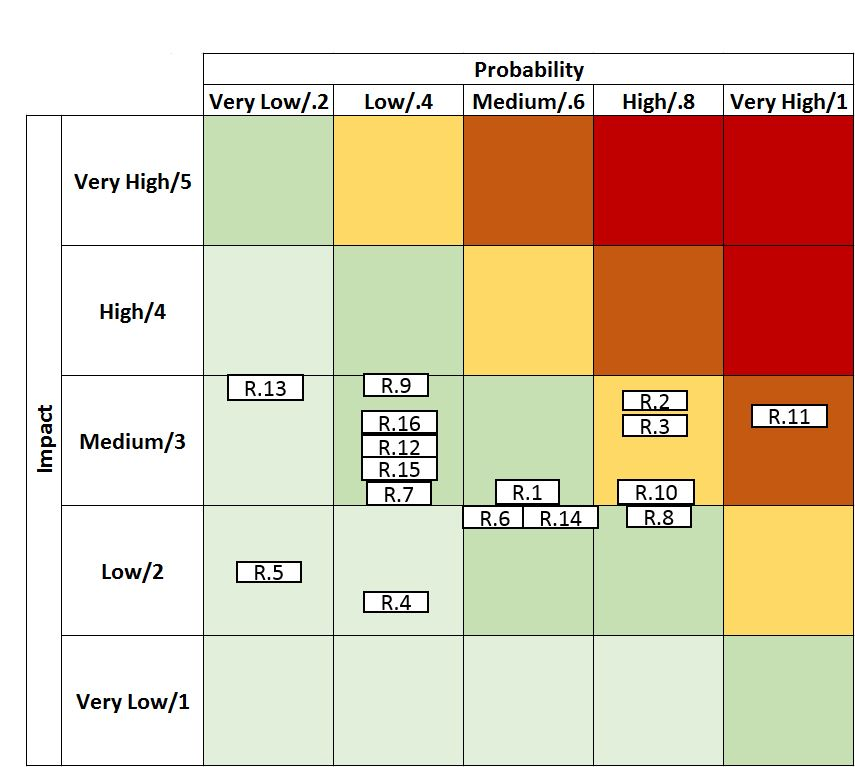
\includegraphics[width=0.9\linewidth]{./images/matrixT1}
	\end{tabular}
	\caption{Risk assessment}
\end{table}

Having done this analysis, the revised situation has to be considered too. It means how the probability and the impact will change once the corresponding response has been executed.

There are also presented the specific actions to take in order to avoid the revised risk and the person responsible to carry them out.

\begin{landscape}

\vspace*{\fill}

	\begin{longtable}{| >{\raggedright\arraybackslash}p{1.4cm}  | >{\raggedright\arraybackslash}p{2.1cm} | >{\centering\arraybackslash}p{3cm} | >{\centering\arraybackslash}p{2cm} | >{\centering\arraybackslash}p{1.4cm} | >{\centering\arraybackslash}p{1.8cm} | >{\raggedright\arraybackslash}p{3.6cm} | >{\raggedright\arraybackslash}p{4cm} |  }
		
		\toprule [2pt]

		\multirow{2}{*}{\textbf{Risk ID}}   &   \multirow{2}{*}{\textbf{\begin{tabular}[c]{@{}l@{}}Revised\\ Probability\end{tabular}}}   &     \multicolumn{3}{| c |}{\textbf{Revised Impact}} &  \multirow{2}{*}{\textbf{\begin{tabular}[c]{@{}l@{}}Revised\\ Score\end{tabular}}}  &  \multirow{2}{*}{\textbf{Owner}}   &	  \multirow{2}{*}{\textbf{Action}}   \\
		
		\cline{3-5}

		\multirow{2}{*}{}  &   \multirow{2}{*}{}   &  \textbf{Scope/Quality}  &   \textbf{Schedule}  &   \textbf{Cost}  &    \multirow{2}{*}{}  & \multirow{2}{*}{} &  \multirow{2}{*}{}   \\  

		\midrule [1.5pt]
		\endhead

		
		R.1 &  Low  &  1  & 2  &  2   &  0.7  & Project Manager & Increase the number of control meetings.
		Allocate more human resources in delayed tasks. \\  

		\hline

		R.2 &  Medium  &  2  &  2 &   2  & 1.2  & Project Manager and Financial Manager  &  Highly periodical cost and expense controls. \\  

		\hline

		R.3 & Low  &  1  &  2  &   1  & 0.5  & Project Manager secretary  & Impart communicative skills courses to team members. Enhance use of collaborative software. \\  

		\hline

		R.4 &  Very Low &  2  & 1  &  1   &  0.3  &  Project Manager & Use all resources that are needed to guarantee the expected innovation. Propose redesigns and alternatives if needed. \\  

		\hline

		R.5 & Very Low  &  1  & 1  &  2   &  0.3  & The manager of the corresponding department  & Maintain contact with scientific and technological centres to be up to date of the last technological improvements. \\  

		\hline

		R.6 &  Low  &  2  & 3  &   1  & 0.7  &  Human Resources Manager  & Interview team members to know their level of satisfaction with their work and request for their suggestions to improve their motivation. \\  

		\hline
		
		R.7 &  Low  & 2   & 1  &   2  & 0.7  &  Quality Manager  & Use higher qualified personnel, and buy better quality control resources. \\  
		
		\hline
		
		R.8 &  Medium  &  1  & 2  &  2   &  1.0  &  Project Manager  & Encourage communication among team members.
		Look for possible causes of conflicts. Establish teambuilding activities. \\  
		
		\hline
		
		R.9 &  Very Low  &  1  & 2  &   4  & 0.5  &  Engineering Department Manager  & Follow the specified design standards. Stick to the available technology. \\  
		
		\hline
		
		R.10 & Low  &  2  & 2  &   2  & 0.8  & Engineering Department Manager  & Establish regular contact with outsourced companies responsible for technological safety. \\  
		
		\hline
		
		R.11 & Medium  &  2  & 2  &  2   &  1.2  &  Project Manager  & Establish weekly meetings between the department responsibles. Enhance the use of organization software. \\  
		
		\hline
		
		R.12 & Very Low  &  1  &  2 &  2   & 0.3  & Project Manager  &  An in-depth research of alternatives to the current members would allow fast solutions. \\  
		
		\hline
		
		R.13 & Very Low  &  3  & 1  &   3  &  0.5  & Quality Manager  & Improve the image that HIRO gives to the European Union. More efficient use of resources. \\  
		
		\hline
		
		R.14 & Low  &  2  &  1 &  2   & 0.7  & Sales Department Manager  & Buy the resources in advance and keep them in stock. \\  
		
		\hline
		
		R.15 & Low  &  2  & 1  &   3  &  0.9  & Sales Department Manager  & Reconsider budget estimations with market variations. \\  
		
		\hline
		
		R.16 & Low  &  2  & 1  &  2   &  0.7  & Software Engineering Manager  & Establish quality inspections of the acquired materials. \\  
		

		\bottomrule[2pt]
		
	\caption{Revised risk identification and assessment}
\end{longtable}

\vspace*{\fill}

\end{landscape}

Finally, the risk assessment with revised risks has been carried out. Note that this time the risks have less probability to happen and less impact if they occur. This is because the taken responses have mitigated the severity of the risks.

\begin{table}[H]
	\centering
	\begin{tabular}{c}
		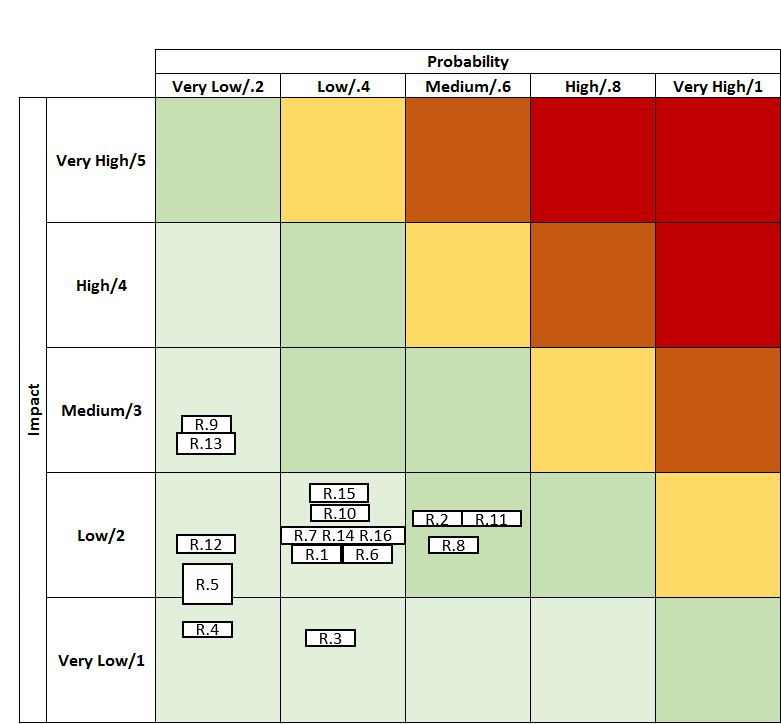
\includegraphics[width=0.9\linewidth]{./images/matrixT2}
	\end{tabular}
	\caption{Revised Risk assessment}
\end{table}